\documentclass[submit]{ipsj}

\usepackage[dvipdfmx]{graphicx}
\usepackage{latexsym}

\def\Underline{\setbox0\hbox\bgroup\let\\\endUnderline}
\def\endUnderline{\vphantom{y}\egroup\smash{\underline{\box0}}\\}
\def\|{\verb|}

\setcounter{page}{1}

\begin{document}

\title{ESSロボットチャレンジ2017}

\etitle{ESS Robot Challenge 2017}

\affiliate{Kyushu}{九州大学}
\affiliate{Kanto}{関東学院大学}
\affiliate{Tokai}{東海大学}
\affiliate{Tokushima}{徳島大学}
\affiliate{TokyoToshi}{東京都市大学}
\affiliate{ChangeVision}{チェンジビジョン}
\affiliate{Shibaura}{芝浦工業大学}

\author{久住 憲嗣}{Kenji Hisazumi}{Kyushu}
\author{元木 誠}{Makoto Motoki}{Kanto}
\author{細合 晋太郎}{Shintaro Hosoai}{Kyushu}
\author{渡辺 晴美}{Harumi Watanabe}{Tokai}
\author{三輪 昌史}{Masafumi Miwa}{Tokushima}
\author{小倉 信彦}{Nobuhiko Ogura}{TokyoToshi}
\author{久保秋 真}{Shin Kuboaki}{ChangeVision}
\author{菅谷 みどり}{Midori Sugaya}{Shibaura}


\begin{abstract}
ESSロボットチャレンジは,本シンポジウムの特別企画であり,「分野・地域を越えた実践的情報教育協働ネットワークenPiT-EMB/PEARL」と共催している.本企画の目的は,自動掃除機ロボットのやマルチコプタ自動航行システムの開発を通し,実践的な組込みシステムの研究・教育を行うことにある.これまで,スプリングスクール,サマースクールを実施し,チュートリアル,スマートモバイルロボット競技,学生企画,ワークショップを開催した.本シンポジウムでは,これまでの結果を踏まえ,デモンストレーション,ポスター,ワークショップを行う.本稿では,本チャレンジの貢献,経緯,企画内容について紹介する.
\end{abstract}

\begin{jkeyword}
教育,スマートモバイルロボット,マルチコプタ
\end{jkeyword}

\begin{eabstract}
ESS Robot Challenge is a special event of ESS and held under the cosponsorship by enPiT-Emb/PEARL. The aim of the event is to provide an open case study for practical research and education for embedded system based on the development contest of automatic vacuum cleaner or automonous multicopter system. On the spring school and the summer school, we carried out tutorials, a smart mobile robot contest, a student session and workshops. In the symposium, the event gives a demonstration, a poster session, and a workshop. The article introduces the contribution, history and events abstract of ESS Robot Challenge.
\end{eabstract}

\begin{ekeyword}
Education, Smart Mobile Robot, Multicopter
\end{ekeyword}

\maketitle

\section{はじめに}
ESSロボットチャレンジは,組込みシステムシンポジウムの特別企画として開催するロボットコンテストである.シンポジウム名が組込みソフトウェアシンポジウムであった頃から継続して実施しており2016年度で13回目となる.

11回目の2014年度に過去10年(10回)を振り返るイベントを実施し\cite{essrc2014},前回の2015年度は未来を考えるために「スマートロボットの実現に向けて〜ソフトウェア・ハードウェアの課題を探る〜」と題したパネルディスカッションを実施し,学会で開催することの意義が,単なるものづくりに留まらず,若手の研究者および技術者の育成,さらに新しい技術へのチャレンジを目指すことを強調できることにあることを確認した\cite{essrc2015}.また,文献\cite{watanabe2016pbl}にもあるように,2016年度で13回目を迎える本チャレンジは,コンテスト型PBL(Project Based Learning)であり, (1)分野を超えた学びの場 (2) 実践的開発経験 (3) コミュニティの形成,に貢献してきたといえる.

本チャレンジは,2013年度より文部科学省「分野・地域を越えた実践的情報教育協働ネットワーク組込みシステム分野連合型PBL(enPiT-Emb/PEARL)」と共催している\cite{enpitweb}\cite{essrcweb}.本共催により,充実した教育環境の提供が可能となり,ロボットチャレンジの成果を研究と結びつけること,大学を超えた学生間の連携を深めることが容易になった.コンテストに先立ち実施するスプリングスクール,サマースクールでは,ロボット開発に必要な知識に加え,学生間で集い実施する学生企画により,学生間の連携を深めている.

また,本チャレンジは2011年度までは小型屋内用飛行船,2012年からは掃除機ロボットを対象としてきたが,2016年度は掃除機ロボットを対象としたスマートロボット競技に加え,飛行ドローンを対象としたマルチコプタ競技も実施する.

以下,2章ではスプリングスクール,サマースクールの概要,3章では学生企画とワークショップ,4章では競技ルールについて紹介し,5章でまとめとする.


\section{スプリング・サマースクール}

ESSロボットチャレンジの事前教育を表\ref{table:schedule}に示す.事前学習は共催のenPiT-Embスプリングスクールおよびサマースクール前半を受講することで行っている.

\subsection{スプリングスクール}

スプリングスクールでは,実践的な組込みシステムを,プロジェクトで開発できる人材育成を目的とし,ロボット開発に必要な基礎知識について演習・実習を交えて学ぶ.講義3日後の5月24日に中間発表会,一週間後の5月27日に課題発表会を実施し,スプリングスクールで学んだことを実践し,不明なことを明らかにし,理解を深める機会を設けている.

%スプリングスクールは開発に必要な基礎知識を学ぶことを目的として実施している.
具体的には,ソフトウェアとハードウェアの設計をロボット制御システムの開発を通して学ぶ.また,プロジェクトマネージメントに関する基礎知識を講義と実践で学べるよう,一週間のミニPBL課題にグループごとに取り組む.
本年度は,昨年度も使用した「iRobotCreate2」というRoombaのプログラマブル教育用ロボットの他に,「Zumo」というキャタピラ式ロボットを導入し,二種類のロボット実践コースを設けた.iRobotCreate2を用いるスマートモバイルロボット競技のコースでは,主に大学院生を対象とし,ロボット制御の基礎演習だけではなく組込みシステム開発方法論に重点をおき課題を実践した.一方で,Zumoを用いるローバトライアル競技のコースでは,主に学部生を対象とし,ロボット開発環境,ロボットに搭載されているセンサーを利用した計測基礎など,組込みプログラミングが初めての学部生にも馴染みやすいように,実装中心の演習を行った.

参加学生数の都合により,同じ大学同士,あるいは,他大学との混成チームを編成したが,学生達はSNS等でコミューニケーションをとりながらミニ分散PBLを実施し,課題の成果をまとめることができた。
全体の約半数の学生がスプリングスクールでの講義・演習内容に興味を持ち,より深く学びたいと感じており、ESSロボットチャレンジにつながるプレセミナーとしての役割を果たす内容であったと考える.

\subsection{サマースクール}

サマースクールは,スプリングスクールの内容を引き継ぎ,各チームで実施してきた開発経験を振り返り,研究にどのように結びつけていくかということを目的として実施している.下記に,サマースクールの講演について,その位置づけおよび内容について概説する.

\begin{table}[ht]
\caption{2017年度スプリング・サマースクール実施スケジュール}
\label{table:schedule}
\centering
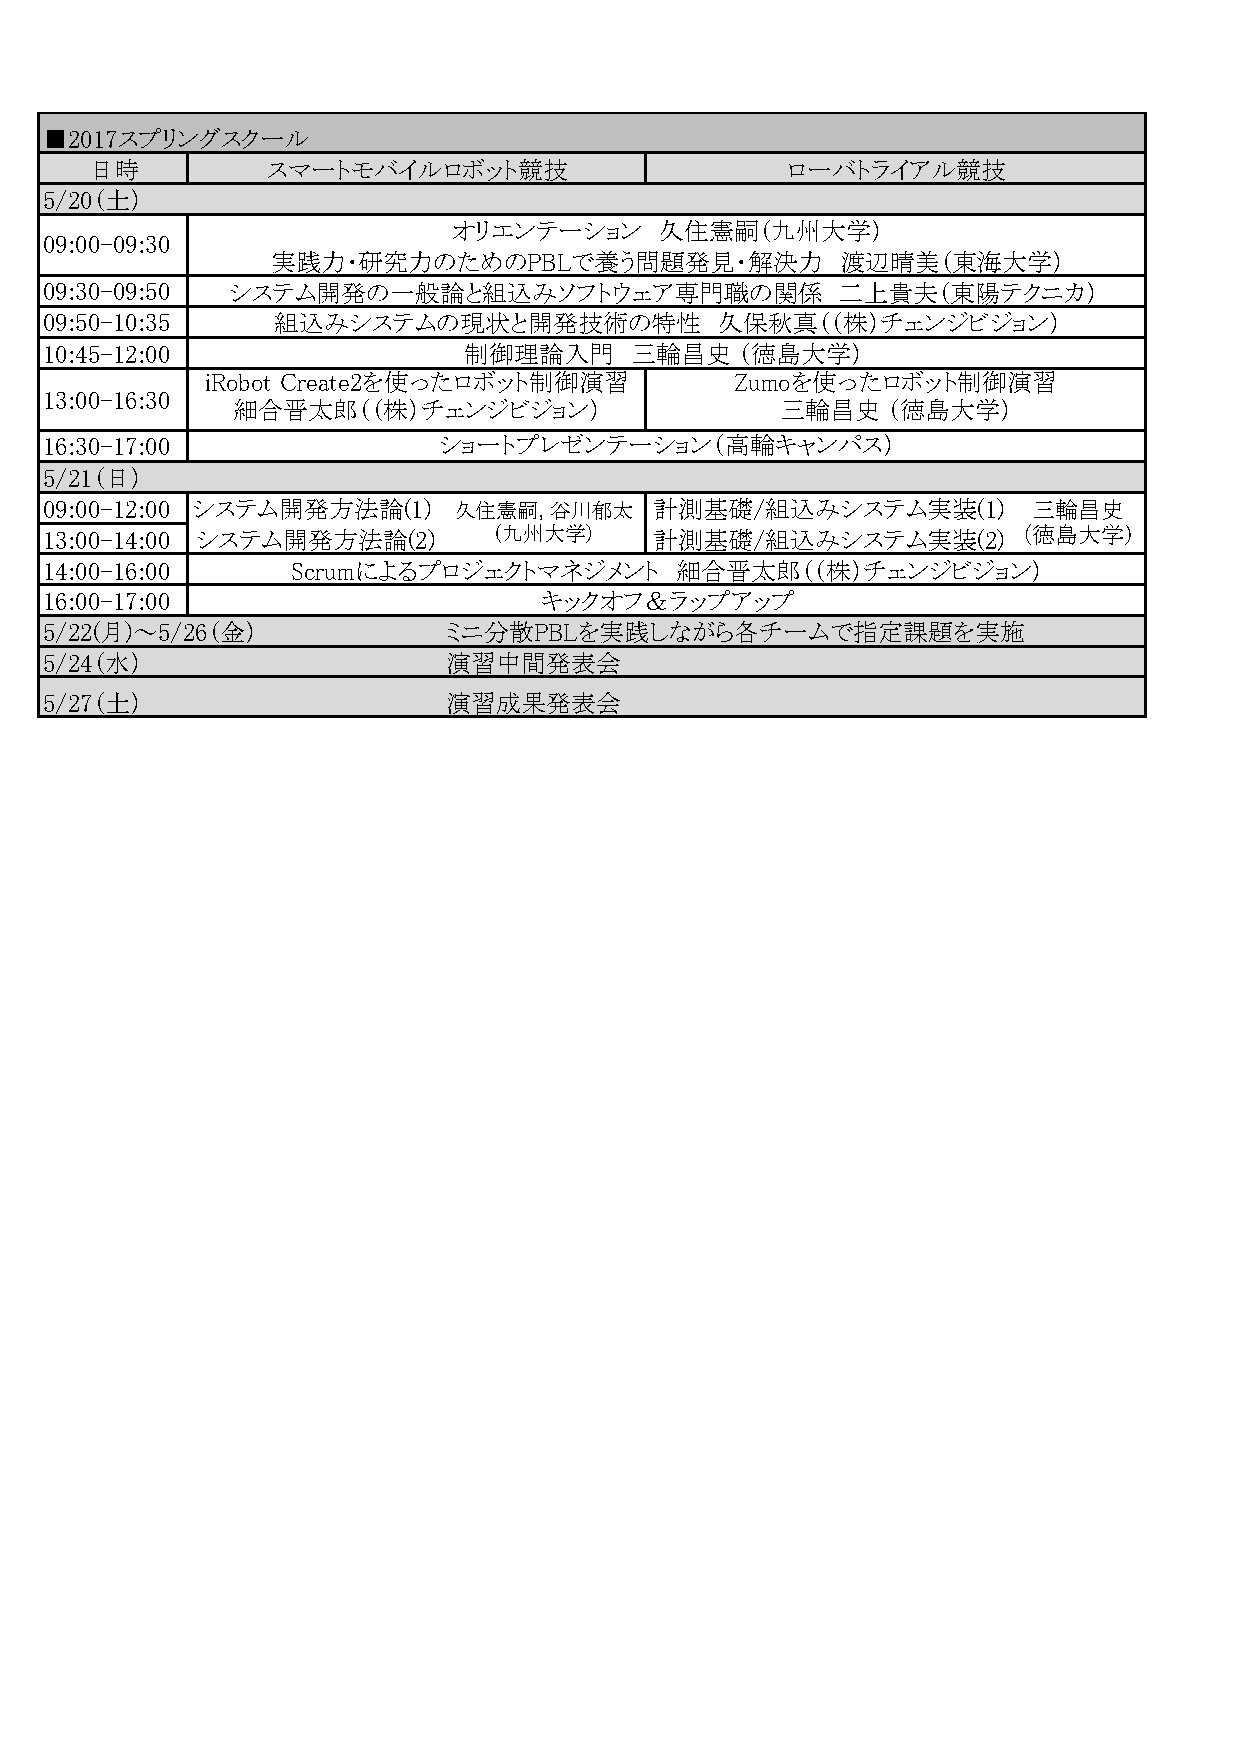
\includegraphics[width=8.5cm]{images/schedule.pdf}
\end{table}

\section{競技ルール}

ESSロボットチャレンジ2016では,掃除機型ロボットを用いたスマートモバイルロボット競技および,飛行ドローンを用いたマルチコプタ競技の2競技で構成される.参加者はいずれかの競技,または両方の競技を選択できる.

\subsection{スマートモバイルロボット競技}
スマートモバイルロボット競技では,サマースクールで実施する中間課題としてコンパルソリ課題,ESSロボットチャレンジ本選において自動掃除課題が課せられる.以下コンパルソリ課題,自動掃除課題について述べる.

\subsubsection{コンパルソリ課題}
\paragraph*{概要}
コンパルソリ課題では5分間であらかじめ与えられた課題を1台の同一のiRobot Create 2を使用してできる限り遂行する.各課題の評価の最高点の合計点をコンパルソリの評点とする.なお,課題ごとに独立したフィールドを設置することとする.

\paragraph*{競技ハードウェア}

iRobot Create2を使用し,制御用デバイスとしてPC,マイコン等を接続することができる.その他のハードウェアの追加は行わないものとする.
\paragraph*{課題実施手順}
課題は以下の手順を規定時間内に繰り返し実施することとする.
\begin{enumerate}
\item 課題を選択する.
\item 課題ごとのフィールドに移動する.
\item 課題実行を審判に宣言する.
\item ロボットを自律的に動作させ課題を遂行する.
\item 課題終了時に審判に宣言する.
\item 審判による評価を待つ.
\item 審判の評価終了宣言に従い次の課題にうつる.
\end{enumerate}

上記(1)〜(5)の実施時間を競技時間に含めるものとし,(5),(6)は競技時間に含めない.(3)を実施中に競技者都合の問題が発生した場合には,競技を放棄し,次の課題に移ることができる.なお,これらの時間は競技時間に含むものとする.また,課題ごとに作られたフィールド上には,測定のためのテープなどが貼られることがある.

\paragraph*{課題}
\begin{enumerate}
\item フィールド上に示した50cm四方の範囲で,180度超信地旋回を反時計回り,時計回り,反時計回り,時計回り,反時計回りに行う.ただし,1回の180度旋回終了後に3秒以上停止する.
\item 1辺2メートルの四角形を描くように時計回りで2周し,走行の軌跡を表示する.ただし,走行軌跡はスタート時の時刻と座標($t_s$, $x_s$, $y_s$)=(0, 0, 0)を基準とし,0.1秒ごとの時刻と座標を課題が終了するまで表示する.
\item 2m四方程度のフィールドを反時計回りに壁沿いを1周した後,ドッキングステーションに帰還する.ただし,壁沿いを1周するまでは,ロボットの一部でも壁から0.5m以上離れてはならない.
\item 2m四方程度のフィールドにまばらに数個程度まかれたゴミを回収する.ただし,ゴミの配置はランダムであり,リトライする場合も再度ランダムに配置される.
\end{enumerate}


\subsubsection{自動掃除課題}
\paragraph*{概要}

iRobot Create2により自律的に掃除を行い掃除の精度を競う競技である.自動掃除課題では規定の時間内(5分〜10分)に環境内を自律的に動作し,フィールドにまかれたゴミを吸い込む.ロボットは最大2台使用することができる.いずれかのロボットが環境中に配置されているドッキングステーションで停止したことをもって,課題終了とする.なお,ドッキングステーションへの到達は充電モードへ切り替わったことにより判定する.課題終了後に吸い込んだゴミの総量等を元に審判が採点する.

\paragraph*{競技ハードウェア}

コンパルソリ競技の構成に加え,iRobot Create 2にセンサなどの追加ハードウェアを追加することができる.ただし,iRobot Create 2の外周よりも10cm以上出てはならない.なお,コンパルソリ競技の構成のみで競技を遂行した場合には加点する.

\paragraph*{実施手順}

\begin{enumerate}
\item セッティングを開始し,機体を大会側が指定した場所(スタート場所)に配置する.
\item 課題実行を審判に宣言する.
\item ロボットが自律的に課題を遂行する.
\item 規定時間終了,もしくは,ドッキングステーションでの停止により課題終了とする.
\end{enumerate}

競技者が中止を判断した場合には,審判に競技中止を宣言した上で,対処を行い,(1)から再開することができる.その際には,内部状態のリセットは行わなくても良いこととするが,必ずスタート場所から再開する必要がある.なお,この時間は競技時間に含むものとする.

\paragraph*{フィールドの形状}
外壁には壁があり,壁に囲まれた内側を環境とする.
\begin{itemize}
\item 環境の大きさは 3[m] x 3[m] ±0.70[m]である.
\item 環境にはゴミがまかれている.
\item フィールド中の特定の箇所に点数の高い加点ゴミがまかれている.
\end{itemize}

\paragraph*{ゴミの仕様}
床にはゴミとしてストロー(φ5mm $\times$ 20mm) がまんべんなくフィールド上に撒かれている.また,場所によってはビーズ(φ8mmプラスチック製)が撒かれている.後者のほうが得点が高い.

\paragraph*{ゴミ排出器}
また,フィールド内に1台のゴミ排出器が設置されている.ゴミ排出器はRaspberry Piで構成されており,WiFiで接続しMQTTを用いて通信する.ロボットがゴミ排出器に特定のメッセージを送信することで,ゴミが排出される.排出されたゴミをすべて吸い取れた場合にはボーナスポイントを付与する.

\paragraph*{フィールド情報の利用}
競技会時にフィールドを使用した試走ができる.ただし,競技会のフィールドの仕様は変更されうるものとする.また,フィールドの形状,ゴミ排出器の位置などの座標情報については,事前に公開した情報以外,自律走行プログラムに与えてはいけないこととする.例えば,試走時にフィールドの計測を行いプログラムに与えて利用するなどである.フィールドを構成する部材の計測についても同様である.なお,情報を利用したことが発覚した場合には0点と評価する.

\paragraph*{競技中の画面表示}
競技中には,ロボットの状態がわかるような画面表示をすること.画面表示には聴衆に見てほしいと思うような,参加者が工夫した点を含めて表示すること.また,大会側が準備した外部のプロジェクターに接続して表示すること.

\paragraph*{評価}
以下の項目から総合的に評価する.
\begin{itemize}
\item 回収したゴミの総量
\item ゲート内ゴミ
\item 追加ハードウェアの有無
\item 画面表示内容のわかりやすさ
\end{itemize}

\subsection{マルチコプタ競技}
マルチコプタ競技では,サマースクールで実施する中間課題として位置計測課題及びホバリング課題,ESSロボットチャレンジ本選において自律航行課題が課せられる.マルチコプタ競技では,いずれの課題においても同様のハードウェアを用いるものとする.以下,マルチコプタ競技のハードウェア構成,位置計測課題,ホバリング課題,自律航行課題について述べる.

\subsubsection{ハードウェア構成}
飛行ドローンとして4枚のプロペラで飛行するクアッドコプターであるMQCX\cite{mqcx}を用いる.図\ref{fig:mqcx}にMQCXの外観を,表\ref{table:mqcx}に主要諸元を示す.

\begin{table}[htb]
\caption{MQCX主要諸元} \label{table:mqcx}
\centering
\begin{tabular}{c|c}\hline
PCBベース最大幅 & 40mm \\
PCBアーム幅 & 4.5mm\\
PCBアーム長 & 105mm\\
モータースパン & 65mm(左右)/92mm(対角)\\
& 最小構成では60mm/85mm\\
最大幅 & 120mm(ローター回転径含む)\\
ローター直径 & 55mm\\
最大合計推力 & 7680g\\
機体重量 & 約34.3g〜(バッテリ含む)\\ \hline
\end{tabular}\\
※機体重量は基板厚/コネクタタイプ/バッテリ容量で変動
\end{table}

\begin{figure}[htb]
\centering
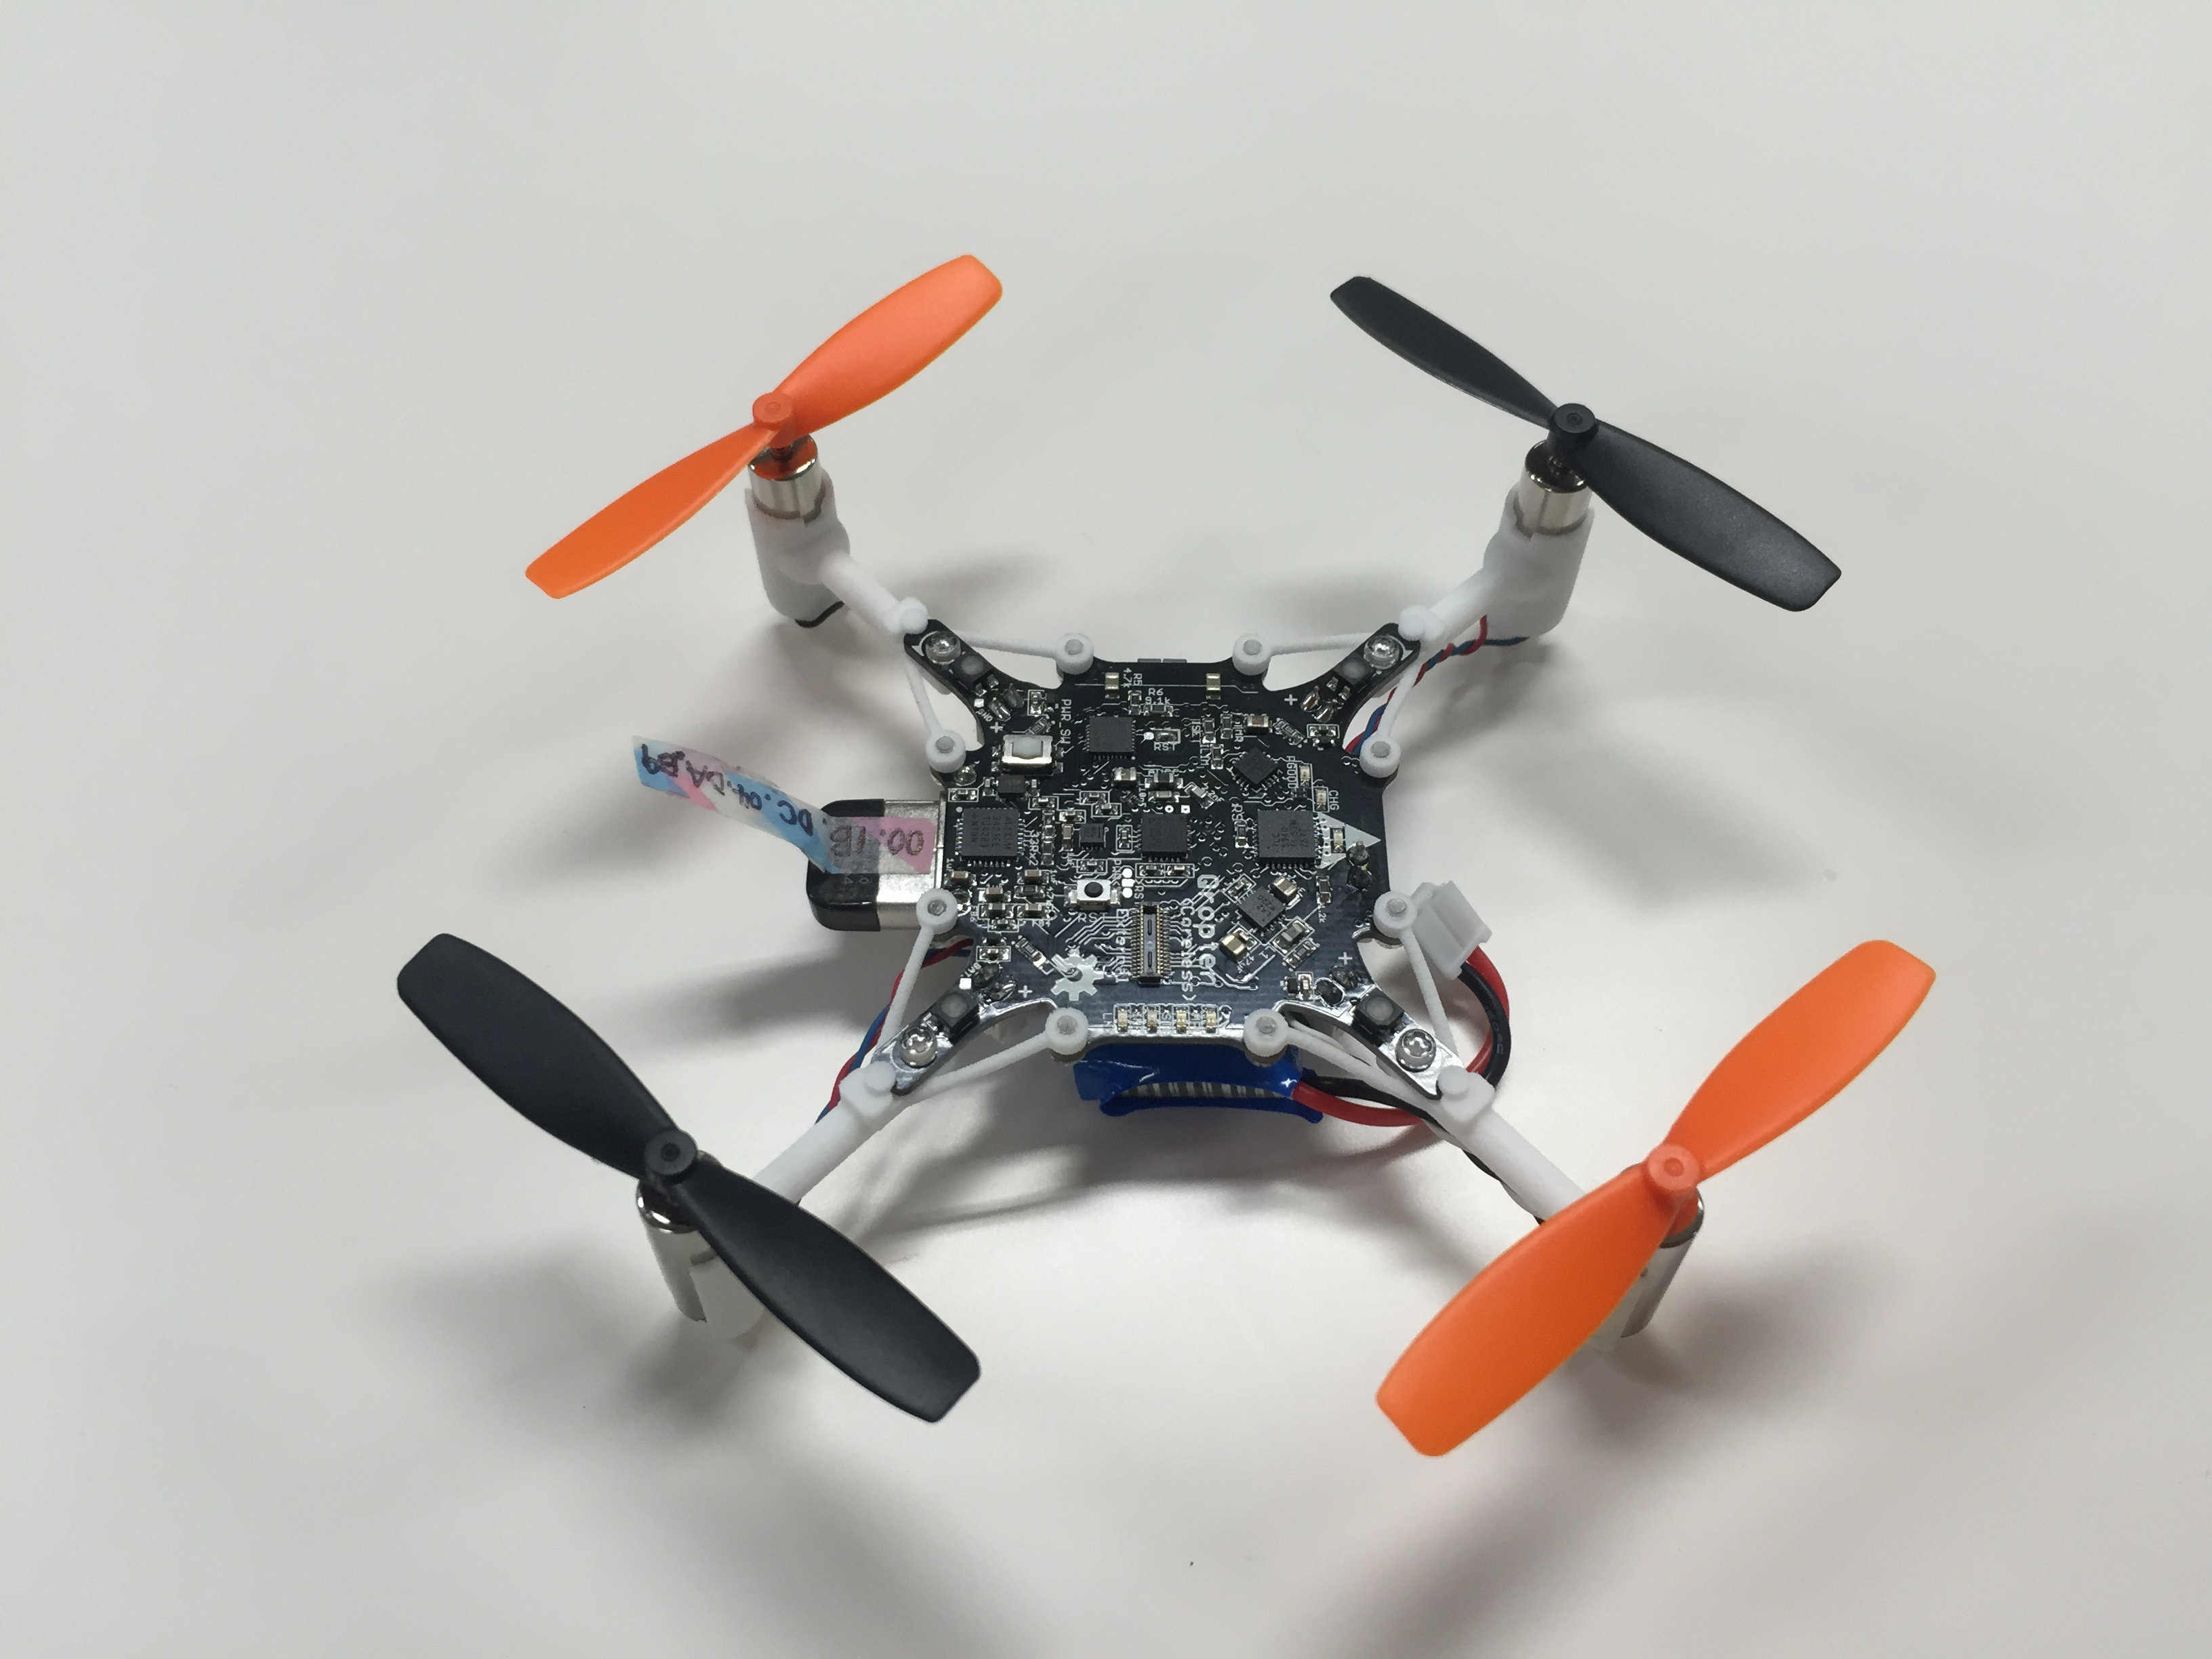
\includegraphics[width=6.5cm]{images/mqcx.jpg}
\caption{MQCX外観} \label{fig:mqcx}
\end{figure}

\subsubsection{位置計測課題}
マルチコプタを用いたプロジェクト型教育やコンテストの課題で用いるのに有効な位置計測方式の提案とそのデモンストレーションを行う.位置計測方式とは,屋内用マルチコプタの自動航行に使用するための,マルチコプタ自体の位置を計測する方式のことである.位置計測チャレンジでは,その設置の容易さや調整の難易度,学習への寄与等も考慮し,評価を行う.

デモストレーションでは,提案された位置計測方式を用いたマルチコプタの実際の飛行,もしくは,飛行体を参加者が動かすことにより行う.それと同時に,位置推定の状況・状態を表示するモニタリングソフトを運用すること.デモストレーションの例としては,例えばあらかじめ設定したコースに対して位置推定ができていることを画面上で示し,さらに可能であれば自律航行を行うことが望ましい.

\subsubsection{ホバリング課題}

自律航行によりホバリングを行い,動作の正確性を競う競技である.この自動航行競技により,高度制御などの飛行技術を評価する.本航行競技では,マルチコプタは以下の競技項目を順次実行していく.
\begin{enumerate}
\item 自動離陸および空中静止(高度制御の確認) 離着陸エリア(1m $\times$ 1m)から離陸し,高度1.5mまで上昇し,空中静止を10秒行う.
\item 離着陸エリア中に着陸する.
\end{enumerate}

\subsubsection{自律航行課題}
自律航行により規定動作を行い,動作の正確性を競う競技である.この自動航行競技により,高度制御・方向制御・直進性能などの飛行技術を確認する.本航行競技では,マルチコプタは以下の競技項目を順次実行していく.

\begin{enumerate}
\item 自動離陸および空中静止(高度制御の確認) 離着陸エリアから離陸し,所定の高度まで上昇,空中静止を10秒行う.
\item 直進飛行(直進性能の確認)空中静止時と同じ高度を維持しつつ,幅3mの飛行エリアを直進する. 折り返しエリア到着後に空中静止する.
\item 90 度旋回(方位制御の確認)折り返しエリアで 90 度回頭後(±15 度程度を維持),空中静止を 10 秒行う.
\item 自動帰還(システムとしての完成度の確認) 離着陸エリアに戻り,着陸する
\end{enumerate}

\paragraph*{フィールド仕様}
5m×5m×4m(天井まで6m85cm)程度の領域を使用することができる.

\section{おわりに}

本稿では,ESSロボットチャレンジ2016について,事前教育のスプリングスクール,サマースクール,学生企画,競技ルールについて紹介した.スプリングスクールでは,ロボット開発に必要な最低限な知識を教育し,サマースクールでは,開発をどのように研究につなげるかということをテーマに実施するとともに,本ロボットチャレンジのコンパルソリ課題を実施した.特に,2016年度から新たに実施しているマルチコプタ競技は,飛行ドローンを対象にしているが故,社会的にも注目度が高い.

また,スプリングスクールとサマースクールを通し,分野・領域が異なる様々な大学・分野の学生達に,共通の知識および問題意識を持たせることができた.特に,サマースクールでは,その共通意識を備えつつ,国内の代表的な研究者研究の講演を通し,研究へ取り組む姿勢が感じ取れるようなカリキュラムとした.その成果は,サマースクールの学生企画の内容,学生の反応から伺うことができ,学生達にとって研究に取り組む姿勢に対して刺激になったと感じている.本シンポジウムのポスターセッション等でその成果が発揮されることであろう.

13年目を迎えたロボットチャレンジを通して,所属機関を越えた教員間,学生間,あるいは学生と教員間の交流が活性化することを期待する.

今後は,高等教育機関に対するPBL教材や教員の育成プログラムの提供など,国内学会として役割を担っていくとともに,本チャレンジから学会開催に相応しい新しい技術が創出されることを期待したい.


\begin{thebibliography}{10}

\bibitem{essrc2014} 渡辺晴美, 久住憲嗣, 三輪昌史, 元木 誠, 小倉信彦, 久保秋 真, 細合晋太郎, 菅谷みどり, 紫合 治: ESSロボットチャレンジ2014, 組込みシステムシンポジウム2014, 組込みシステムシンポジウム2014論文集, pp.134--139, 2014.

\bibitem{essrc2015}	渡辺晴美, 久住憲嗣, 三輪昌史, 元木 誠, 小倉信彦, 久保秋 真, 細合晋太郎, 菅谷みどり, 紫合 治: ESSロボットチャレンジ2015, 組込みシステムシンポジウム2015, 組込みシステムシンポジウム2015論文集, pp.112--116, 2015.

\bibitem{watanabe2016pbl} 渡辺晴美, 三輪昌史, 元木 誠, 小倉信彦, 久保秋 真, 細合晋太郎, 菅谷みどり, 久住憲嗣: 学会実施のコンテスト型PBLによる組込みシステム教育, 日本工学教育協会工学教育, Vol.64, No.3, pp.41--46, 2016.

\bibitem{enpitweb} enPiT-Emb/PEARLホームページ, \urlj{http://www.qito.kyushu-u.ac.jp/project/pearl} (2016.9.15).

\bibitem{essrcweb} ESSロボットチャレンジホームページ, \urlj{http://www.qito.kyushu-u.ac.jp/ess/} (2016.9.15).

\bibitem{mqcx}
魔法の大鍋: マルチコプタ(online),
\urlj{http://blog.eldhrimnir.com/wordpress/?page\_id=3749}
(2016.9.15).

\end{thebibliography}

\end{document}

